\chapter{Application on Sirius Storage Ring}

This final chapter is dedicated to the application of the theory and code presented and discussed in the previous chapters on Sirius storage ring. A few tests were performed with measured~\glspl{orm} using the electron beam in the storage ring. The stored current used during the measurements was $\SI{10}{\milli\ampere}$, which is a value that provides a good accuracy for~\gls{bpm} readings and the beam stability is guaranteed as well.

The~\gls{orm} measurement procedure is controlled by~\gls{sofb}, the same software that controls the orbit correction system and the bipolar method is used. Both horizontal and vertical kicks variations used for the measurements were $\Delta \theta_x = \Delta \theta_y = \SI{15}{\micro\meter}$ and the variation in~\gls{rf} frequency was $\Delta f_{\mathrm{rf}} = \SI{80}{\hertz}$. These variations are intermediate in the sense that they provide a compromise between sufficient orbit distortion for accurate~\gls{bpm} measurements and keeping small variations to avoid non-linear effects. Nominally, the peak orbit distortions at~\glspl{bpm} for half of correctors variations are $\Delta x = \SI{196}{\micro\meter}$ and $\Delta y = \SI{134}{\micro\meter}$. The peak horizontal distortion for a $\SI{40}{\hertz}$ variation in~\gls{rf} frequency is $\Delta x = \SI{38}{\micro\meter}$. The~\gls{orm} typical measurement time for Sirius storage ring is $40$ minutes.

The beam orbit was measured  with the~\glspl{bpm} during $\SI{10}{\second}$ and the average variation obtained for each plane was $\sigma_{\mathrm{BPM}, x} = \SI{162(6)}{\nano\meter}$ and $\sigma_{\mathrm{BPM}, x} = \SI{233(7)}{\nano\meter}$.

% \begin{figure}
% \centering
% \begin{subfigure}[t]{0.49\textwidth}
% 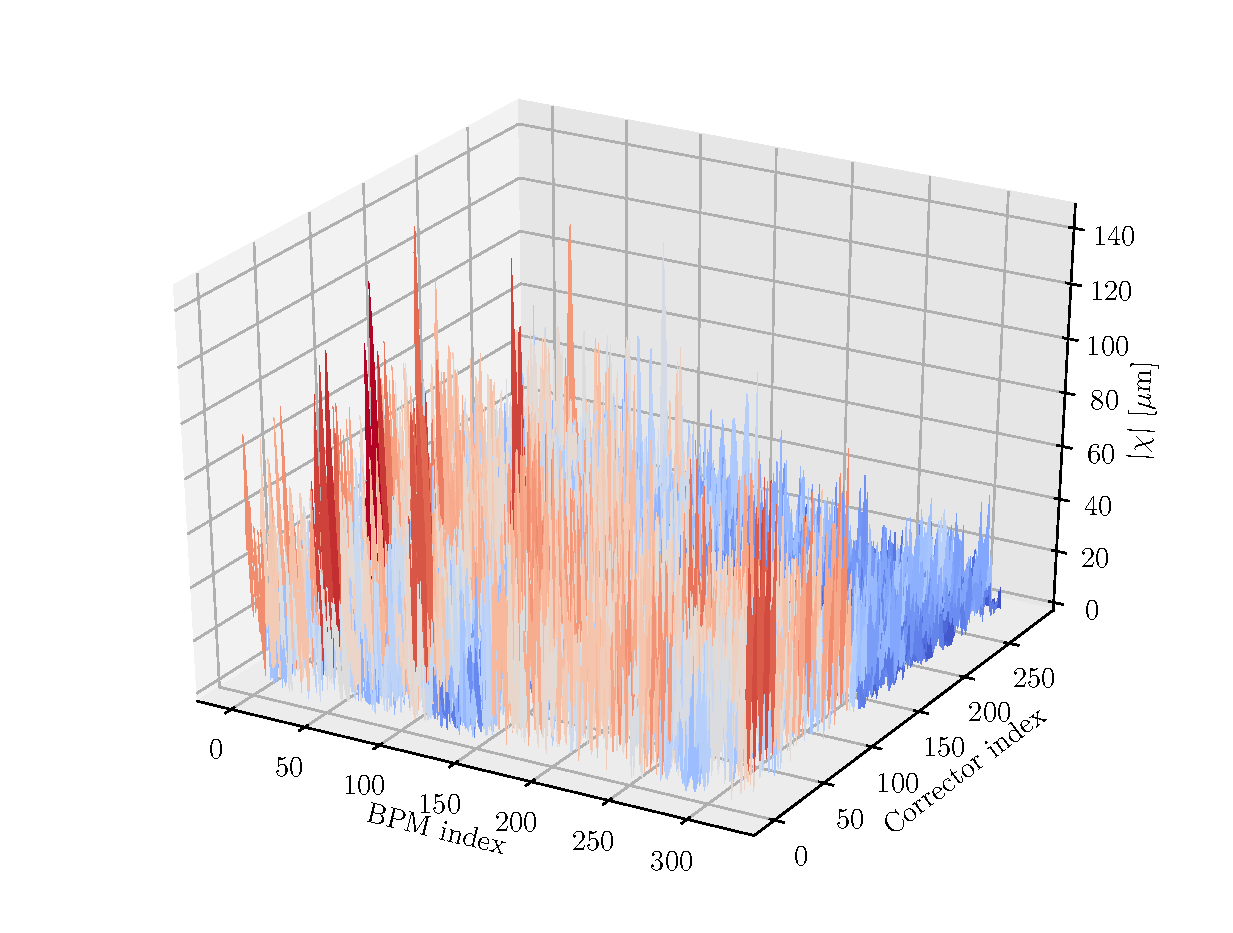
\includegraphics[width=1.0\textwidth]{figures/loco_surface_iter0_before.eps}
%     \caption{Before.}
%     \label{subfig:ondiag}
% \end{subfigure}
%  \begin{subfigure}[t]{0.49\textwidth}
% 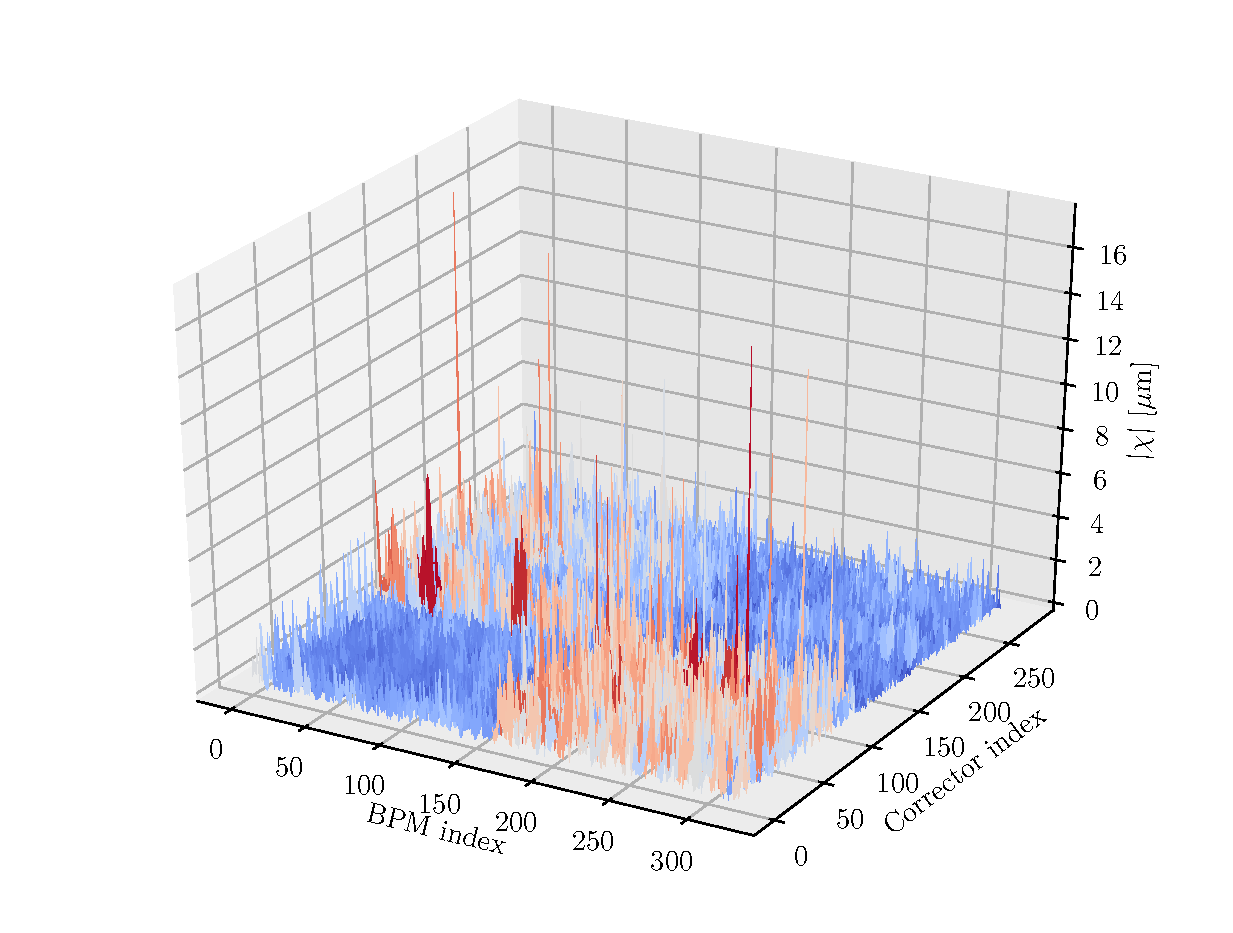
\includegraphics[width=1.0\textwidth]{figures/loco_surface_iter0_after.eps}
%     \caption{After.}
%     \label{subfig:offdiag}
% \end{subfigure}
% \caption{\gls{orm} error distribution before and after LOCO fitting.}
% \label{fig:hist}
% \end{figure}

%The kicks used for conversion are $\Delta \theta_x = \Delta \theta_y = \SI{15}{\micro\meter}$.

% \begin{figure}
% \centering
% \begin{subfigure}[t]{0.49\textwidth}
% \includegraphics[width=1.0\textwidth]{figures/histogram_iter0_ondiag.eps}
%     \caption{On-diagonal.}
%     \label{subfig:ondiag}
% \end{subfigure}
%  \begin{subfigure}[t]{0.49\textwidth}
% \includegraphics[width=1.0\textwidth]{figures/histogram_iter0_offdiag.eps}
%     \caption{Off-diagonal.}
%     \label{subfig:offdiag}
% \end{subfigure}
% \caption{\gls{orm} error histograms.}
% \label{fig:hist}
% \end{figure}

\section{Tests on Measured Data}

\subsection{Determine LOCO Configuration}\label{subsec:loco_config}
From tests with simulated model and jacobian matrix analysis discussed in Chapter~\ref{chap:code_studies}, the chosen LOCO configuration was: include the parameters presented in Table~\ref{tab:fit_params} in the fitting, use~\gls{lm} method as the minimization algorithm setting $\lambda = 10^{-3}$ initially, use the $\Delta K$ constraints with weight $c_{\Delta K} = 10^{3}$ and remove only the last singular value for pseudo-inversion of LOCO jacobian matrix. 

In order to check if this setup is appropriated for LOCO analysis in the real Sirius storage ring a simple test was performed. Without any optics or coupling corrections applied in the storage ring, an~\gls{orm} was measured and it was used to apply the LOCO method with two setups: without any modification (using~\gls{gn} method and no constraint on $\Delta K$) and with the chosen configuration described previously. The initial $\chi$ for the measured~\gls{orm} was $\SI{24.6}{\micro\meter}$ and for both LOCO fittings, $\chi$ converged to values close to $\SI{0.9}{\micro\meter}$. However there is a great difference between the two calibrated models regarding the quadrupole deviations from the nominal values. As discussed in the Chapter~\ref{chap:loco}, without constraints on $\Delta K$, the LOCO process tries to minimize $\chi$ without concern on the quadrupoles deviations, which may lead to large excursions in these parameters due to the quasi-degeneracies in LOCO jacobian. With constraints on $\Delta K$, the convergence path for $\chi$ is changed also minimize the step size of quadrupole deviations. This difference in the fitting behavior can be revealed with a plot of $\chi$ versus the euclidean norm of quadrupole variations over iterations, as presented in Figure~\ref{fig:chi_vs_dkl}.
\begin{figure}
\centering
\includegraphics[width=0.75\textwidth]{figures/chi_versus_dk.eps}
\caption{$\chi$ versus the euclidean norm $||\Delta K/K||$ throughout 10 LOCO iterations. The black dashed line corresponds to $\chi = \SI{908}{\nano\meter}$, the value used as reference for convergence.}
\label{fig:chi_vs_dkl}
\end{figure}

The comparison of final fit variations for the 270 quadrupoles in Sirius storage ring in this test is plotted in Figure~\ref{fig:dkl_compare}. The variations reaching $\SI{7.5}{\%}$ are clearly unrealistic, based on available magnetic measurements data of these quadrupoles, which indicates a good gradient field quality with variations as low as $\SI{0.1}{\%}$. The solution obtained with constraints demands much less of quadrupole variations and also adjusts the measured~\gls{orm} in the same level. The variations obtained for the other parameters included in the fitting agrees for the two setups within the error bars, which was expected since basically the major difference is related to the constraints on quadrupoles strengths.
\begin{figure}
\centering
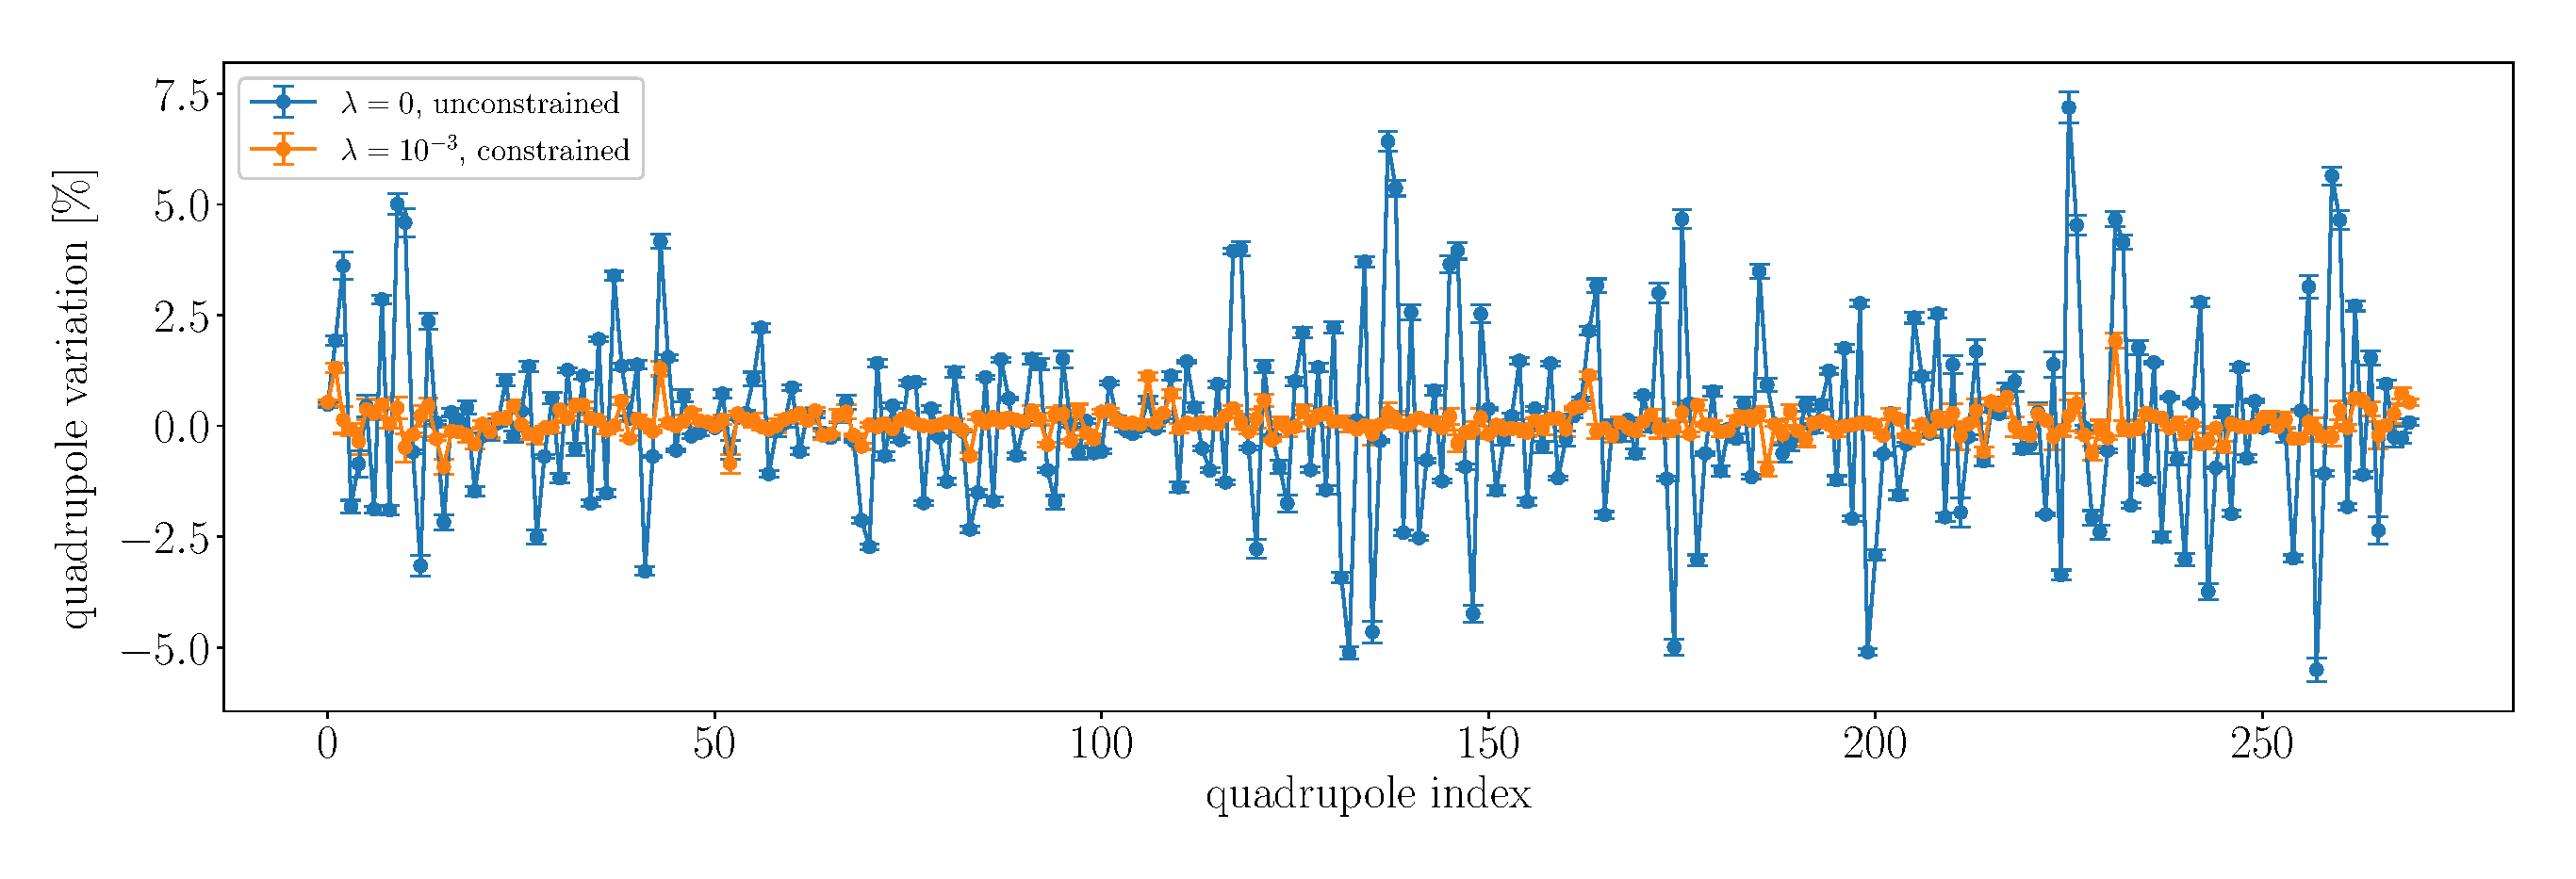
\includegraphics[width=1.0\textwidth]{figures/delta_kl_comparison_better.eps}
\caption{Comparison of quadrupoles variations obtained from LOCO with two calculation methods.}
\label{fig:dkl_compare}
\end{figure}

It is important to point out that the convergence criteria for $\chi$ should avoid the cases of over-fitting. In addition to save the LOCO running time, the most important reason is to prevent the method from increasing the quadrupoles strengths to produce a negligible reduction in $\chi$. The over-fitting is more serious for the unconstrained case, since each iteration may produce large variations on quadrupoles but it may also be a problem even for the constrained case, since accumulated small step sizes may also produce large and unnecessary variations in the final values. The convergence criteria can be controlled by defining the minimum acceptable change in the residue, given by $\chi_{\mathrm{step}}$ and the minimum level for the residue, $\chi_{\mathrm{min}}$. For the LOCO fittings performed in Sirius storage ring, the values used was $\chi_{\mathrm{step}} = \SI{10}{\nano\meter}$ and $\chi_{\mathrm{step}} = \SI{250}{\nano\meter}$, where the value for $\chi_{\mathrm{min}}$ was defined based on Sirius \glspl{bpm} accuracy. The final residue of $\SI{908}{\nano\meter}$ obtained in these fittings is still $3.6$ times greater than the \gls{bpm} accuracy and the explanation for this limit of convergence will be given throughout this chapter. Nevertheless, obtain a calibrated model with an \gls{orm} that agrees with the measured in the sub-$\mu$m level already corresponds to a very good fitting.

\subsection{Fit Parameters Variation}
As mentioned in~\cite{safranek1997}: ``\textit{the easiest way to determine how much the set of fit parameters vary due to random errors in the measurements is simply to measure many~\gls{orm}, analyze each one separately, and see how much variation there is between fit parameters for the different data sets}''. Therefore, to determine the variations of fit parameters presented in Table~\ref{tab:fit_params}, the aforementioned procedure was applied in Sirius storage ring, where 10~\glspl{orm} were measured sequentially. 

The~\gls{loco} analysis was performed in these 10 measured~\glspl{orm} with the configuration described in Subsection~\ref{subsec:loco_config} and the results are organized in Table~\ref{tab:fit_var}. The average initial residue for these 10 realizations was $\chi_{\mathrm{initial}} = \SI{9.2(4)}{\micro\meter}$ and after the convergence the average final residue was $\chi_{\mathrm{final}} = \SI{1.04(2)}{\micro\meter}$. For each calibrated model, the optical functions and its variations in this set of 10 values were also calculated. The results are organized in Table~\ref{tab:twiss_var}. For each parameter, the~\gls{std} variation obtained in the 10 LOCO realizations was used to define the corresponding error bars.
\begin{table}
    \centering
    \caption{Variations in fit parameters from LOCO analysis of 10 ORM measurements performed in Sirius storage ring.}
    \label{tab:fit_var}
    \begin{tabular}{cccc}
        \toprule\toprule
        Parameter & std variation & peak-to-valley variation & Unit \\
        \hline
        Quadrupole Relative Strength     & 0.13 & 0.32 & \% \\  
        H. BPM Gain             & 0.06 & 0.27 & \%\\
        H. Corrector Gain       & 0.18 & 1.03 & \%\\
        V. BPM  Gain             & 0.07 & 0.35 & \%\\
        V. Corrector Gain       & 0.21 & 1.14 & \%\\
        Skew Quadrupole Absolute Strength& \num{1.3e-4} & \num{6.2e-4} & $\SI{}{\meter^{-1}}$\\
        BPM roll angle                & 0.25 & 1.31 & $\SI{}{\milli\radian}$ \\
        \bottomrule\bottomrule
    \end{tabular}
\end{table}
\begin{table}
    \centering
    \caption{Variations in lattice functions obtained from calibrated models after LOCO analysis of 10 ORM measurements performed in Sirius storage ring.}
    \label{tab:twiss_var}
    \begin{tabular}{cccc}
        \toprule\toprule
        Lattice function & std variation & peak-to-valley variation & Unit \\
        \hline
        $\beta_x$ & \num{0.17}& \num{0.86} & \%\\
        $\beta_y$ & \num{0.14} & \num{0.99}& \% \\
        $\eta_x$ & \num{0.26} & \num{1.36} & \SI{}{\milli\meter}\\
        $\eta_y$ & \num{0.62} & \num{2.62} & \SI{}{\milli\meter} \\
        \bottomrule\bottomrule
    \end{tabular}
\end{table}

The variations for the dispersion functions are calculated as absolute values because $\eta_x$ is zero in the straight sections, so it is not possible to divide the variations by the average values and then obtain a finite relative variation. To compare the variations in Table~\ref{tab:twiss_var}, the average and~\gls{std} of $\eta_x$ around the Sirius storage ring is $\SI{2.1}{\cm}$ and the peak-to-valley value is $\SI{8.3}{\cm}$. In the case of betatron functions, which always assumes positive values by definition, it is possible to obtain the relative variations.


\subsection{Finding Planted Errors}


\section{Linear Optics and Coupling Correction}

\begin{figure}
\centering
\begin{subfigure}[t]{0.49\textwidth}
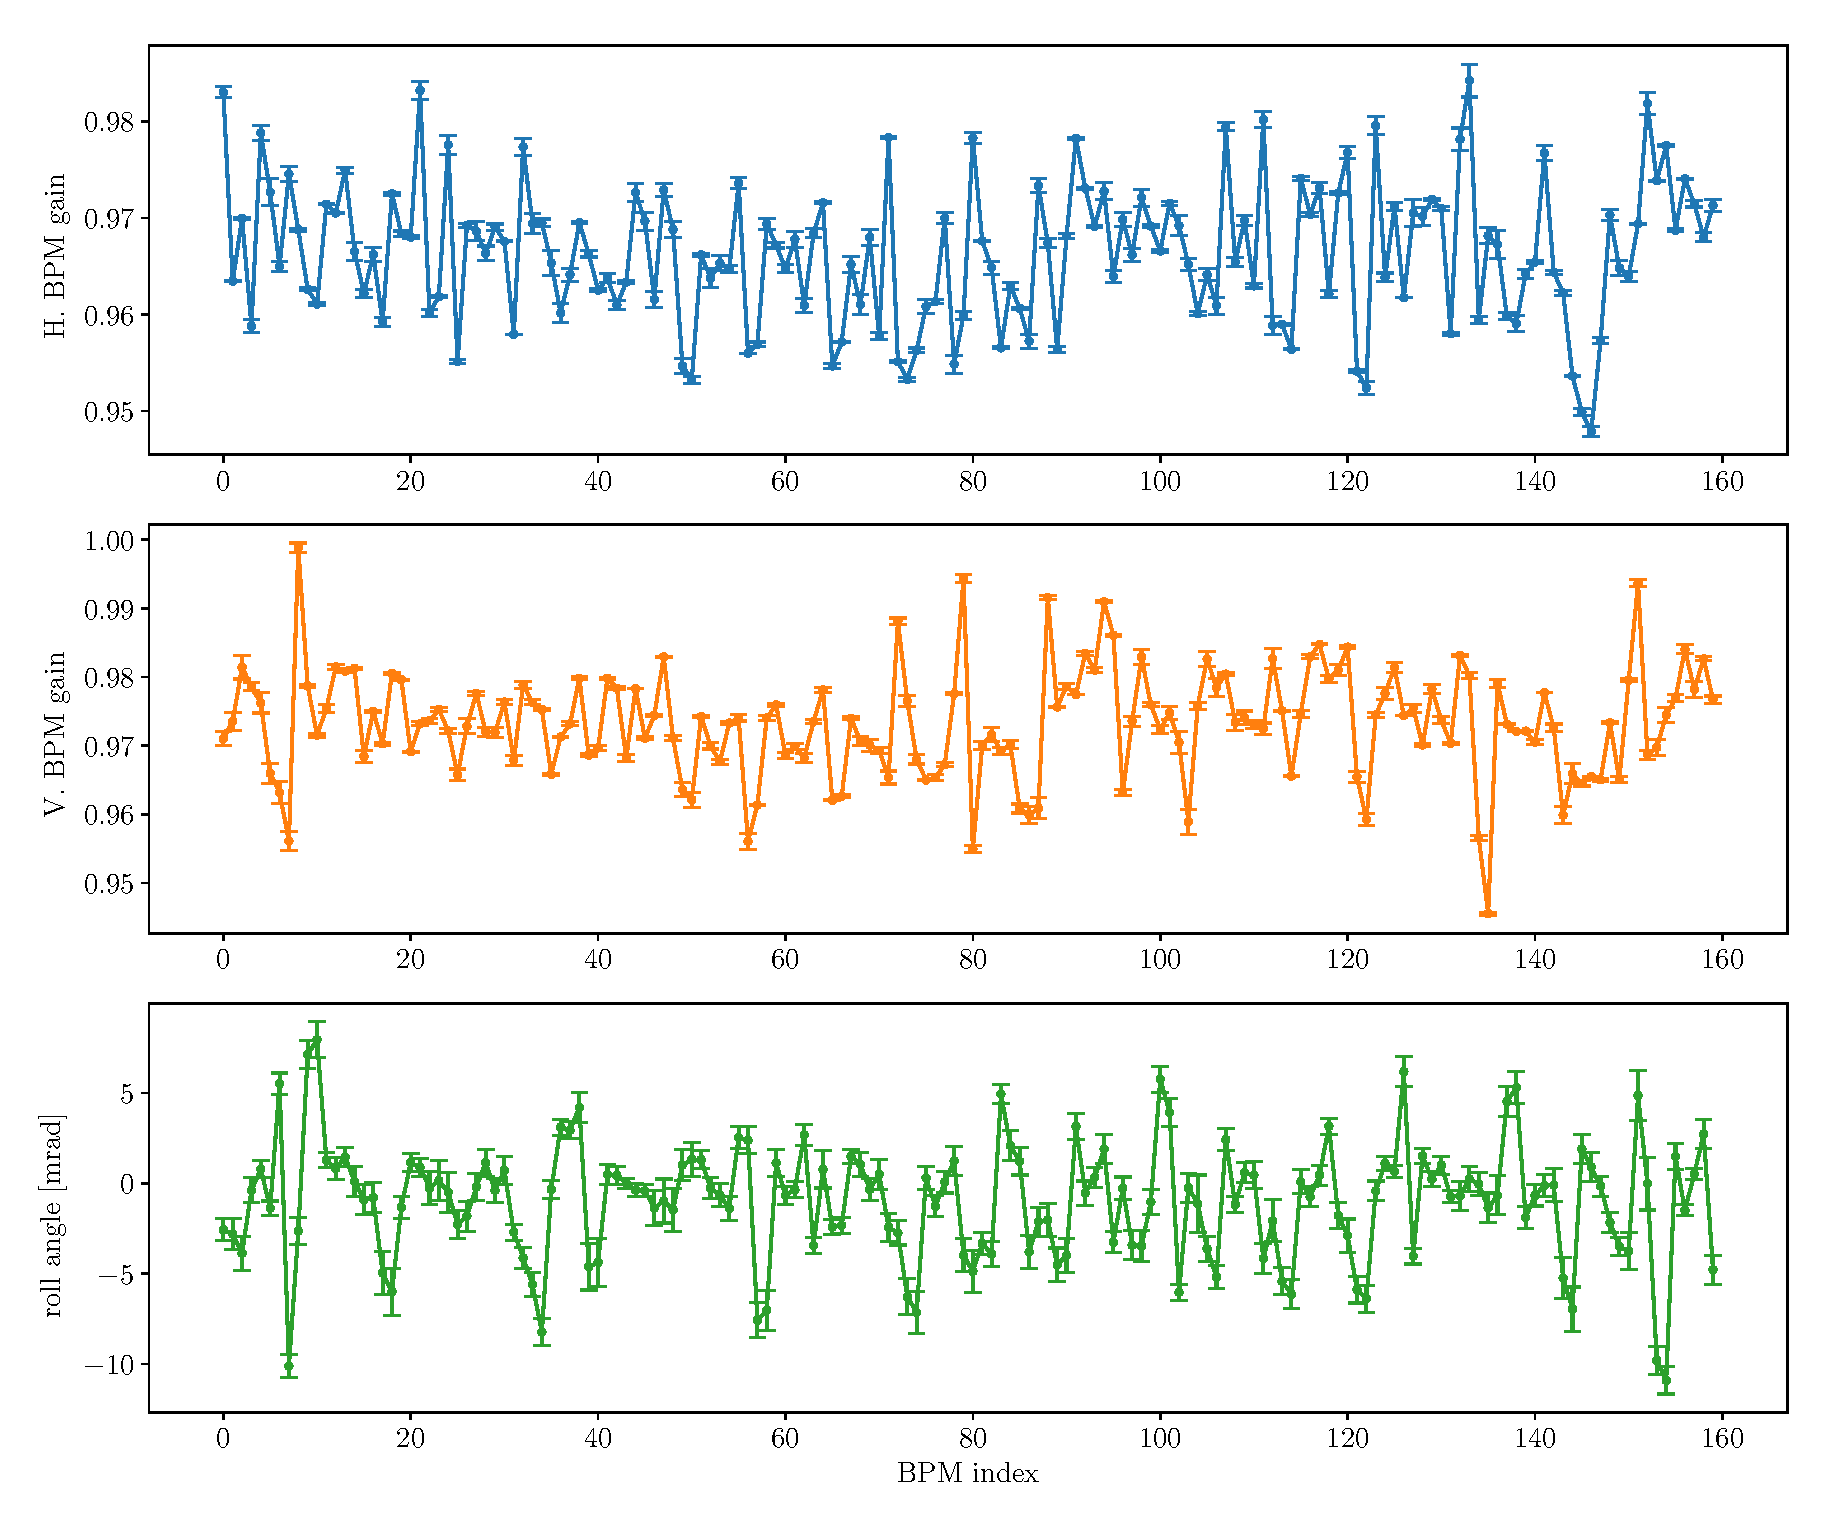
\includegraphics[width=1.0\textwidth]{figures/bpm_gains_iter0.eps}
    \caption{BPM gains and roll angles.}
    \label{subfig:bpm_fit}
\end{subfigure}
 \begin{subfigure}[t]{0.49\textwidth}
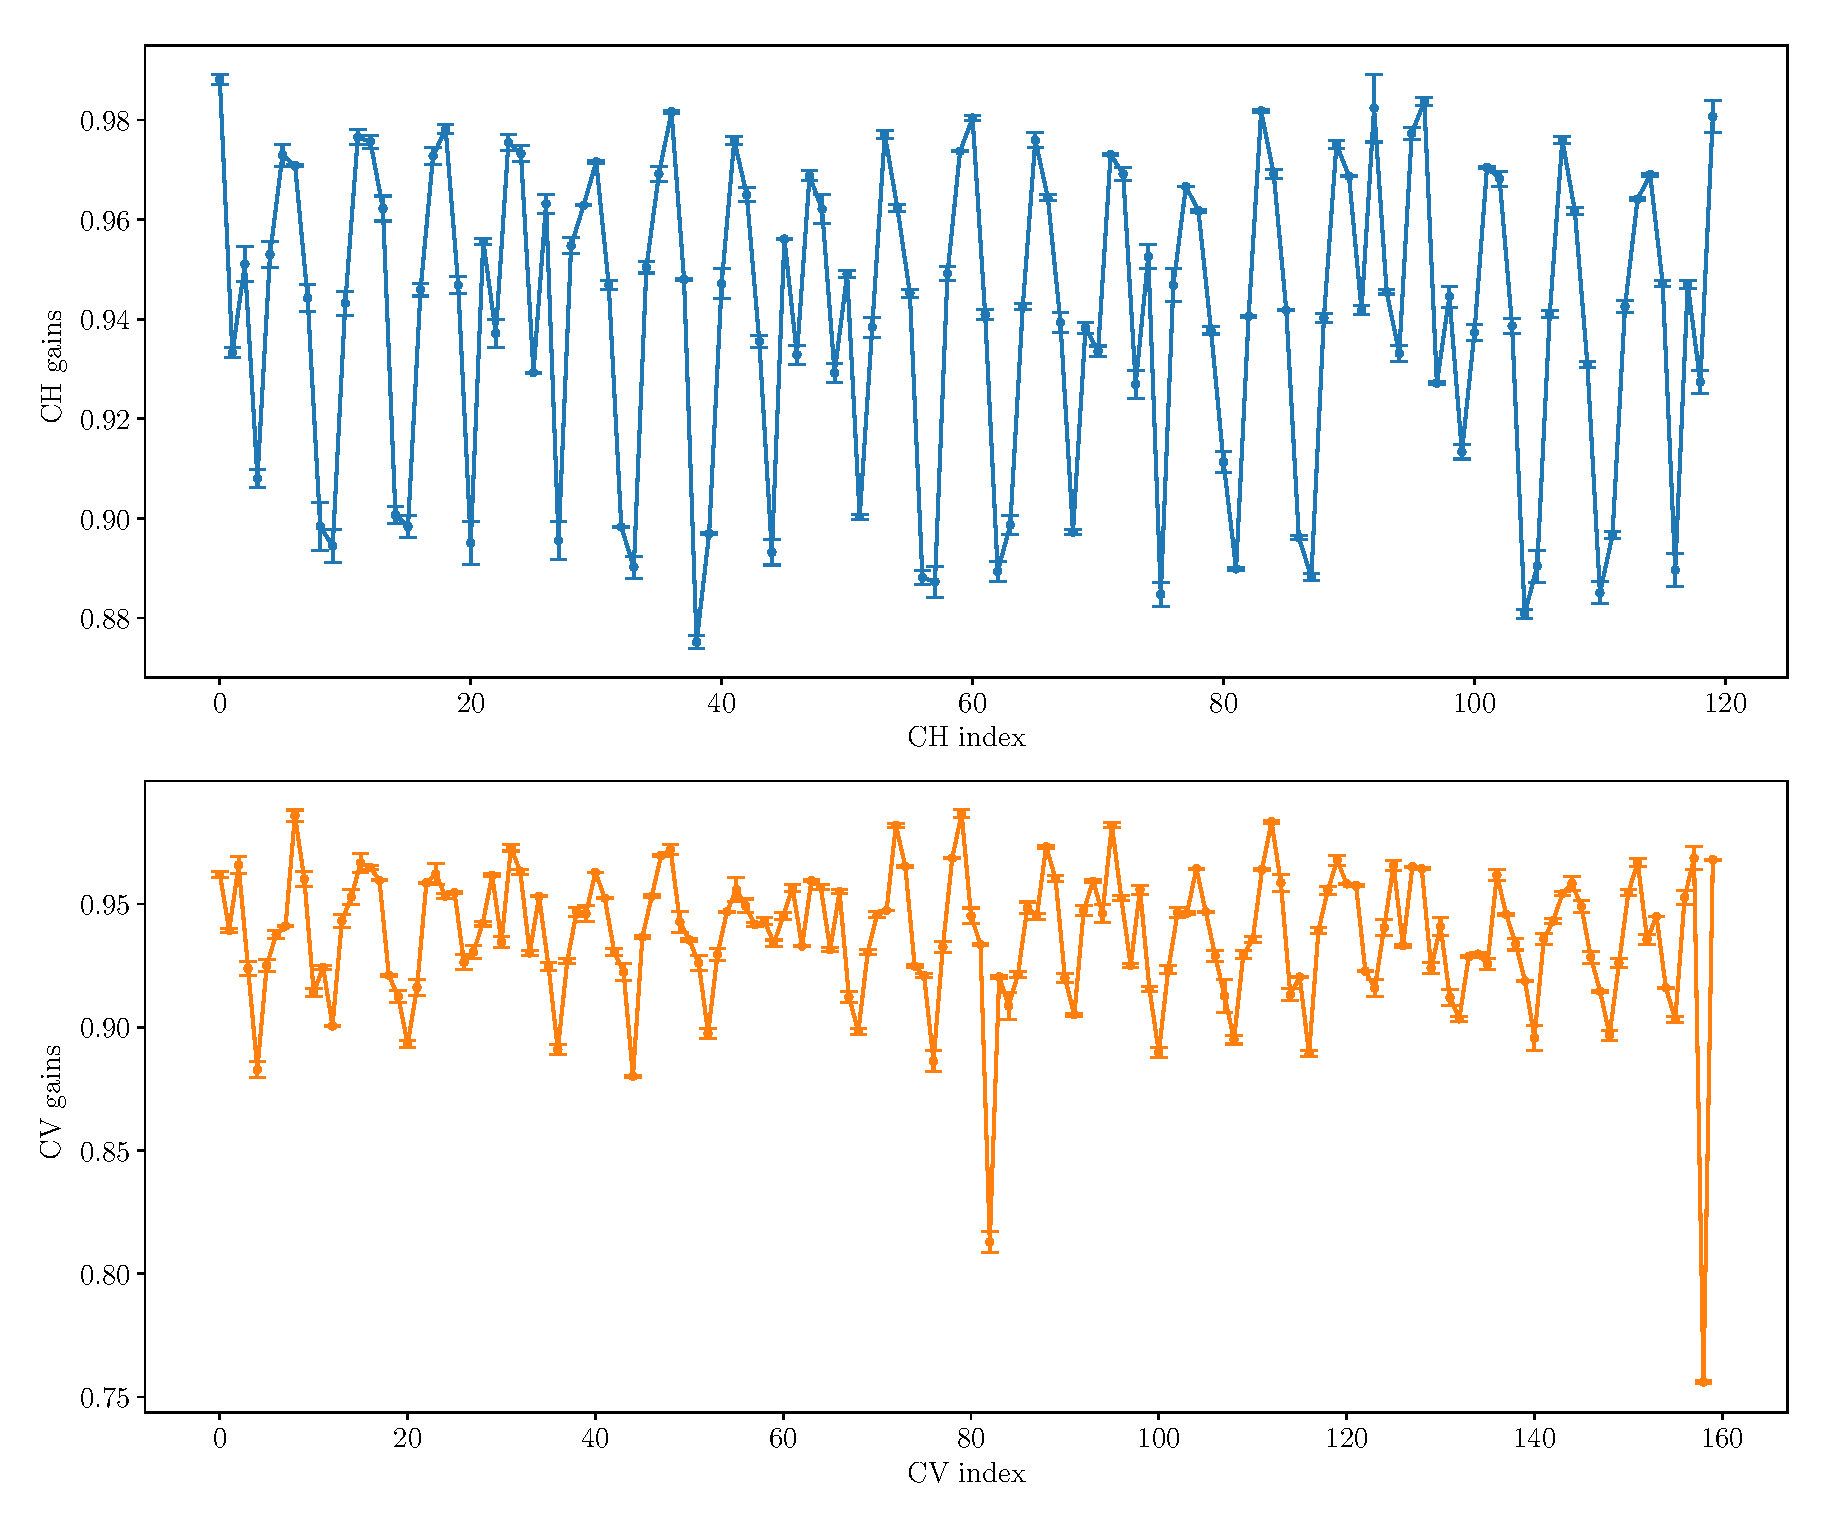
\includegraphics[width=1.0\textwidth]{figures/corr_gains_iter0.eps}
    \caption{Correctors gains.}
    \label{subfig:corr_fit}
\end{subfigure}
\caption{Fitted values for BPM gains, roll errors and correctors (CH and CV) gains.}
\label{fig:gain_fit}
\end{figure}

\begin{figure}
\centering
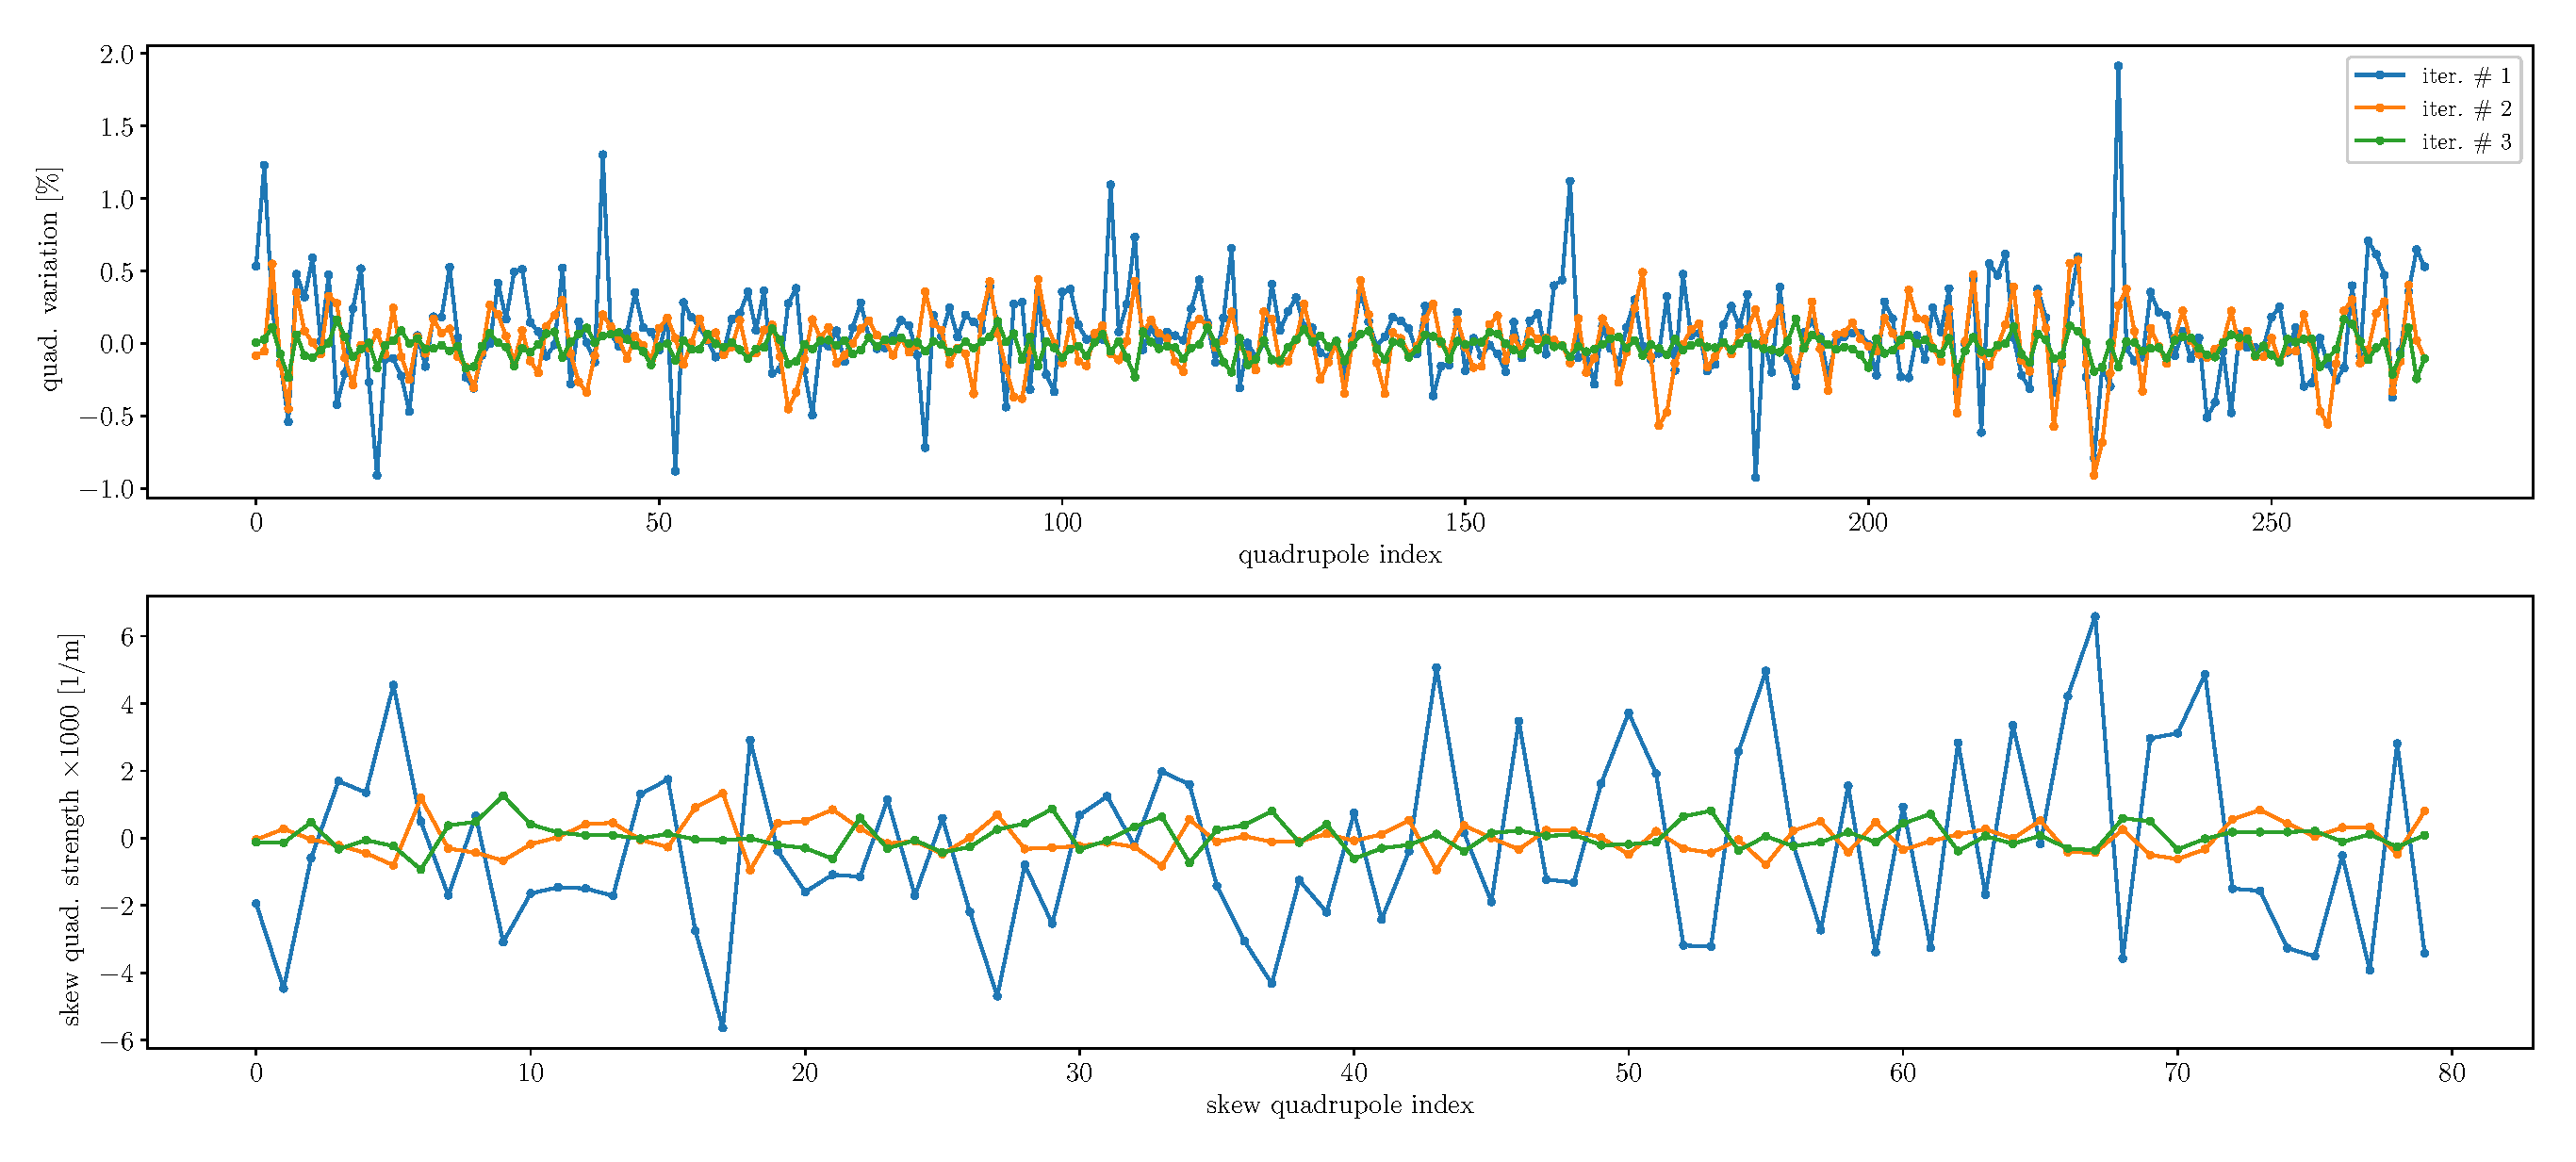
\includegraphics[width=1.0\textwidth]{figures/loco_quad_skewquad_corrections.eps}
\caption{Normal and skew quadrupoles corrections for three LOCO iterations.}
\label{fig:loco_corrections}
\end{figure}

\begin{figure}
\centering
\begin{subfigure}[t]{0.49\textwidth}
\includegraphics[width=1.0\textwidth]{figures/surface_before_loco.pdf}
    \caption{Before.}
    \label{subfig:ondiag}
\end{subfigure}
 \begin{subfigure}[t]{0.49\textwidth}
\includegraphics[width=1.0\textwidth]{figures/surface_after_loco.pdf}
    \caption{After.}
    \label{subfig:offdiag}
\end{subfigure}
\caption{Orbit response matrix error surface before and after LOCO corrections.}
\label{fig:hist}
\end{figure}

\begin{figure}
\centering
\includegraphics[width=1.0\textwidth]{figures/histogram_loco_iterations.pdf}
\caption{Histogram for the errors between measured and nominal orbit response matrices for each LOCO iteration. The blue data refers to the measured ORM without corrections applied. The orange data was obtained after the first application of LOCO corrections. The green data is related to the second and last LOCO round applied.}
\label{fig:histogram}
\end{figure}

\begin{figure}
\centering
\includegraphics[width=1.0\textwidth]{figures/nominal_measured_after_before_loco.eps}
\caption{Orbit Response Matrix rows for the first CH and CV. The blue curve is the nominal ORM, the orange curve represents the measured ORM before LOCO corrections and the green curve is from measured ORM after LOCO.}
\label{fig:orm_rows}
\end{figure}

\begin{figure}
\centering
\includegraphics[width=1.0\textwidth]{figures/nominal_measured_dispersion_after_before_loco.eps}
\caption{Dispersion measurements and difference from nominal values (blue curves), before (orange curves) and after (green curves) LOCO corrections.}
\label{fig:disp_error}
\end{figure}


\section{Independent Measurements}
\subsection{Betatron Function}
\subsection{Betatron Coupling}

\begin{figure}
\centering
\begin{subfigure}[t]{0.49\textwidth}
\includegraphics[width=1.0\textwidth]{figures/coupling_before_loco.eps}
    \caption{Before.}
    \label{subfig:coup_before}
\end{subfigure}
 \begin{subfigure}[t]{0.49\textwidth}
\includegraphics[width=1.0\textwidth]{figures/coupling_after_loco.eps}
    \caption{After.}
    \label{subfig:coup_after}
\end{subfigure}
\caption{Global betatron coupling before and after LOCO corrections.}
\label{fig:global_coupling}
\end{figure}

\subsection{Horizontal Dynamic Aperture}
\begin{figure}
\centering
\includegraphics[width=0.75\textwidth]{figures/xdynamic_aperture.eps}
\caption{Comparison of horizontal dynamic aperture measurement before and after LOCO corrections.}
\label{fig:xdynap}
\end{figure}

Setting $5\%$ as the beam loss limit to estimate the dynamic aperture, after the application of LOCO corrections on linear optics and coupling, the horizontal dynamic aperture was increased from $\SI{7.6}{\milli\meter}$ to $\SI{8.3}{\milli\meter}$, which is an optimization of approximately $10\%$.






% \section{Orbit response matrix}
% \section{Transverse Linear Coupling}
% \section{Betatron Function}
% \section{Dispersion Function}
% % \section{Emittance}
% \section{Dynamical Aperture}
% \section{Injection Efficiency}
